% ============================================================================
%  Rapport -- quantum-vs-classical-classifier
%  Compilation : pdflatex rapport.tex (deux fois pour les références)
%  Les tableaux et figures de ../results/ sont inclus automatiquement s'ils existent
%  (générés par : python run_benchmark.py).
% ============================================================================
\documentclass[11pt,a4paper]{article}

\usepackage[utf8]{inputenc}
\usepackage[T1]{fontenc}
\usepackage[french]{babel}
\usepackage{lmodern}
\usepackage{microtype}
\usepackage[margin=2.5cm]{geometry}
\usepackage{amsmath,amssymb}
\usepackage{booktabs}
\usepackage{graphicx}
\usepackage{xcolor}
\usepackage{tikz}
\usetikzlibrary{babel}   % évite le conflit entre babel (français) et les circuits TikZ
\usepackage{quantikz}   % dessin de circuits ; fournit \ket et \bra
\usepackage{csquotes}
\usepackage[hidelinks]{hyperref}

\graphicspath{{../results/}}
\newcommand{\resultats}{../results}
\newcommand{\afaire}[1]{\textcolor{orange!80!black}{\textbf{À compléter :} #1}}
% Inclut un fichier de résultats s'il existe, sinon affiche un rappel.
\newcommand{\inclureresultat}[2]{%
  \IfFileExists{\resultats/#1}{#2}{\afaire{lancer \texttt{python run\_benchmark.py} pour générer \texttt{results/#1}.}}}

\title{\textbf{Classifieurs quantiques et classiques :\\ une comparaison expérimentale}\\[0.4em]
\large Projet 1 -- Série « IA et informatique quantique »}
\author{Prénom Nom\\ Master 1 Informatique et Mobilité -- Université de Haute-Alsace}
\date{\today}

\begin{document}
\maketitle

\begin{abstract}
L'apprentissage automatique quantique promet d'exploiter la superposition et l'intrication
pour classer des données. Nous comparons deux modèles quantiques -- un classifieur quantique
variationnel (VQC) et une machine à vecteurs de support à noyau quantique -- à trois références
classiques, sur des jeux de données identiques et avec des métriques identiques. Sur les
petits problèmes étudiés, les modèles quantiques simulés n'atteignent pas la précision des
meilleurs modèles classiques, pour un coût de calcul nettement supérieur, mais le VQC s'en
approche avec très peu de paramètres. \afaire{mettre à jour ce résumé avec les résultats finaux.}
\end{abstract}

\tableofcontents
\newpage

% ----------------------------------------------------------------------------
\section{Introduction}

Les ordinateurs quantiques actuels, dits NISQ (\emph{Noisy Intermediate-Scale Quantum}),
comptent quelques dizaines à quelques centaines de qubits bruités. Les algorithmes
\emph{variationnels}, qui confient à un optimiseur classique le réglage d'un circuit quantique
paramétré, sont la piste la plus étudiée pour en tirer parti à court terme, notamment en
apprentissage automatique \cite{mitarai2018,schuld2020}.

\paragraph{Question.} Sur des tâches de classification binaire de petite taille, un
classifieur quantique fait-il mieux, aussi bien ou moins bien qu'un classifieur classique,
et à quel coût ?

\paragraph{Démarche.} Plutôt que de chercher un cas favorable au quantique, nous suivons les
recommandations de Bowles \emph{et al.} \cite{bowles2024} : mêmes données, même prétraitement,
références classiques solides, et rapport explicite des coûts.

% ----------------------------------------------------------------------------
\section{Notions d'informatique quantique}

\subsection{Le qubit et la mesure}
Un qubit est un vecteur unitaire de $\mathbb{C}^2$ :
\begin{equation}
  \ket{\psi} = \alpha\ket{0} + \beta\ket{1}, \qquad |\alpha|^2 + |\beta|^2 = 1 .
\end{equation}
Sa mesure donne $0$ avec probabilité $|\alpha|^2$ et $1$ avec probabilité $|\beta|^2$.
Un registre de $n$ qubits vit dans un espace de dimension $2^n$ : c'est cette croissance
exponentielle qui rend la simulation classique coûteuse au-delà de quelques dizaines de qubits.

\subsection{Portes et rotations}
Les portes quantiques sont des matrices unitaires. La rotation
\begin{equation}
  R_Y(\theta) = \begin{pmatrix} \cos\frac{\theta}{2} & -\sin\frac{\theta}{2} \\
                                \sin\frac{\theta}{2} & \cos\frac{\theta}{2} \end{pmatrix}
\end{equation}
envoie $\ket 0$ sur un état où $P(1) = \sin^2(\theta/2)$. Son paramètre continu en fait
l'équivalent quantique d'un poids de réseau de neurones.

\subsection{Intrication}
Le circuit de la figure~\ref{fig:bell} produit l'état de Bell
$\ket{\Phi^+} = \tfrac{1}{\sqrt 2}(\ket{00} + \ket{11})$ : chaque qubit est aléatoire, mais
les deux mesures coïncident toujours. Cet état ne peut pas s'écrire comme un produit de deux
états à un qubit.

\begin{figure}[h]
\centering
\begin{quantikz}
\lstick{$\ket{0}$} & \gate{H} & \ctrl{1} & \meter{} \\
\lstick{$\ket{0}$} &          & \targ{}  & \meter{}
\end{quantikz}
\caption{Préparation et mesure de l'état de Bell $\ket{\Phi^+}$.}
\label{fig:bell}
\end{figure}

\subsection{Encodage des données}
Une donnée $x \in [0,\pi]^n$ est encodée par $U(x) = \bigotimes_{i=1}^n R_Y(x_i)$
(\emph{encodage en angles}). Il faut donc un qubit par variable, d'où la réduction de dimension
préalable par analyse en composantes principales (ACP).

% ----------------------------------------------------------------------------
\section{Modèles comparés}

\subsection{Classifieur quantique variationnel (VQC)}
Le modèle applique l'encodage $U(x)$, puis $L$ couches entraînables $W(\boldsymbol\theta)$
(rotations générales sur chaque qubit suivies d'un anneau de portes CNOT), et mesure
l'observable $Z$ sur le premier qubit (figure~\ref{fig:vqc}) :
\begin{equation}
  f(x;\boldsymbol\theta, b) =
  \bra{0}U(x)^\dagger W(\boldsymbol\theta)^\dagger Z_0\, W(\boldsymbol\theta) U(x)\ket{0} + b
  \in [-1-b,\,1+b].
\end{equation}
La classe prédite est $\operatorname{sign} f$. Les paramètres minimisent l'erreur
quadratique moyenne avec étiquettes $y \in \{-1, +1\}$, par l'optimiseur Adam sur des
mini-lots. Les gradients se calculent sur matériel réel grâce à la règle du
\emph{parameter shift} \cite{mitarai2018}. Le nombre de paramètres est $3nL + 1$.

\begin{figure}[h]
\centering
\begin{quantikz}
\lstick{$\ket{0}$} & \gate{R_Y(x_1)} & \gate[3]{W(\boldsymbol\theta)} & \meter{} \rstick{$\langle Z\rangle$} \\
\lstick{$\ket{0}$} & \gate{R_Y(x_2)} &                                 &  \\
\lstick{$\ket{0}$} & \gate{R_Y(x_3)} &                                 &
\end{quantikz}
\caption{Architecture du VQC (exemple à trois qubits).}
\label{fig:vqc}
\end{figure}

\subsection{SVM à noyau quantique}
Le circuit sert ici d'\emph{application de caractéristiques} $x \mapsto \ket{\phi(x)}$
\cite{havlicek2019}. Le noyau
\begin{equation}
  k(x, x') = \left|\langle \phi(x') | \phi(x) \rangle\right|^2
\end{equation}
est estimé en appliquant $V(x)$ puis $V(x')^\dagger$ et en mesurant la probabilité de
retrouver $\ket{0\cdots0}$. La carte $V$ alterne encodages $R_Y$, chaîne de CNOT et
encodages $R_Z$. Un SVM classique est ensuite entraîné sur la matrice de Gram. En simulation
exacte, nous calculons directement les vecteurs d'état, ce qui donne le même noyau avec
$n$ simulations au lieu de $n^2$.

\subsection{Références classiques}
Régression logistique, SVM à noyau gaussien (RBF) et perceptron multicouche à deux couches
cachées de 16 neurones (scikit-learn).

% ----------------------------------------------------------------------------
\section{Protocole expérimental}

\begin{itemize}
  \item \textbf{Données} : \texttt{moons} et \texttt{circles} (synthétiques, 200 points,
        bruit 0{,}15), \emph{Iris} restreint à deux classes, \emph{Breast Cancer Wisconsin}.
  \item \textbf{Prétraitement} : standardisation, ACP vers $n$ dimensions ($n$ = nombre de
        qubits), puis mise à l'échelle dans $[0, \pi]$. Ces transformations sont apprises
        sur l'ensemble d'entraînement uniquement.
  \item \textbf{Découpage} : 70\,\% entraînement, 30\,\% test, stratifié, graine fixée.
  \item \textbf{Métriques} : accuracy, score F1, temps d'entraînement, nombre de paramètres.
  \item \textbf{Simulation} : \texttt{default.qubit} (PennyLane), état exact, sans bruit.
\end{itemize}

% ----------------------------------------------------------------------------
\section{Résultats}

\subsection{Jeu \texttt{moons}, 2 qubits}

\begin{table}[h]
\centering
\inclureresultat{moons_2q.tex}{\input{\resultats/moons_2q.tex}}
\caption{Résultats sur \texttt{moons} (test, 60 points). Le SVM n'a pas de nombre fixe de paramètres.}
\label{tab:moons}
\end{table}

\begin{figure}[h]
\centering
\inclureresultat{moons_2q.png}{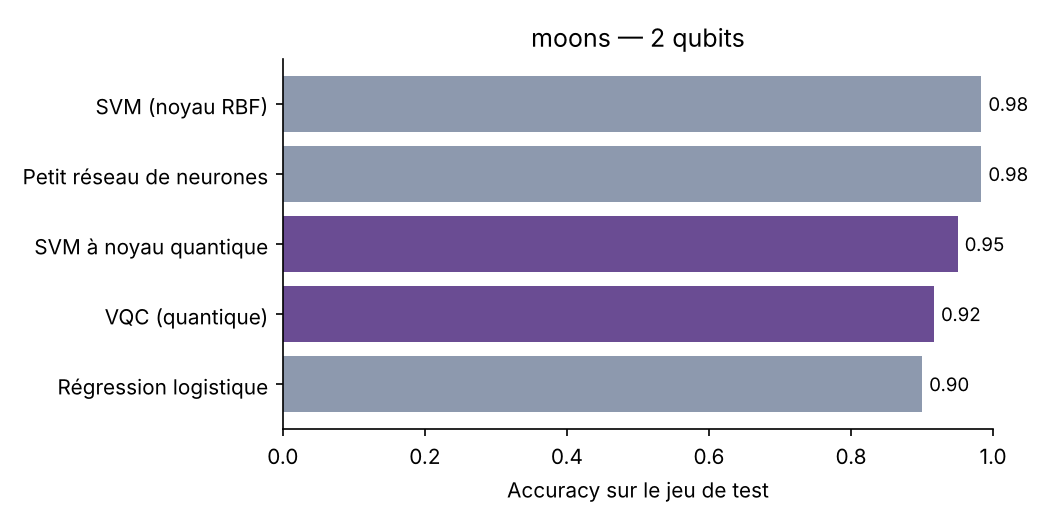
\includegraphics[width=0.8\linewidth]{moons_2q.png}}
\caption{Accuracy sur le jeu de test (violet : modèles quantiques).}
\end{figure}

\subsection{Jeu \emph{Breast Cancer}, 4 qubits}

\begin{table}[h]
\centering
\inclureresultat{breast_cancer_4q.tex}{\input{\resultats/breast_cancer_4q.tex}}
\caption{Résultats sur \emph{Breast Cancer} réduit à 4 composantes principales.}
\label{tab:bc}
\end{table}

\subsection{Étude systématique}
\afaire{faire varier le nombre de qubits (2 à 8), de couches (1 à 5) et la taille du jeu
d'entraînement ; tracer l'accuracy et le temps d'entraînement en fonction de ces paramètres.}

% ----------------------------------------------------------------------------
\section{Bruit et exécution sur matériel réel}
\afaire{(1) répéter les expériences avec un nombre fini de mesures (\emph{shots}) ;
(2) ajouter un modèle de bruit (Qiskit Aer) ; (3) exécuter le VQC entraîné sur un processeur
IBM Quantum et comparer l'accuracy à la simulation.}

% ----------------------------------------------------------------------------
\section{Discussion}

\paragraph{Précision.} Sur ces petits problèmes, les modèles classiques atteignent une
accuracy au moins égale à celle des modèles quantiques. Ce résultat est cohérent avec les
études systématiques récentes \cite{bowles2024}.

\paragraph{Coût.} Simuler un circuit coûte $\mathcal{O}(2^n)$ en mémoire. Sur matériel réel,
chaque évaluation demande des centaines de mesures, et le calcul du gradient deux évaluations
par paramètre.

\paragraph{Expressivité et entraînabilité.} Le VQC obtient de bons résultats avec très peu
de paramètres, mais ses circuits profonds souffrent de \emph{plateaux stériles} : le gradient
s'annule exponentiellement avec le nombre de qubits \cite{mcclean2018}.

\paragraph{Limites de l'étude.} Données de faible dimension, simulation sans bruit, peu de
réglage des hyperparamètres. \afaire{compléter.}

% ----------------------------------------------------------------------------
\section{Conclusion}
\afaire{résumer les résultats, répondre à la question posée en introduction, et ouvrir sur
les projets suivants (QAOA, agent de génération de circuits, décodage des erreurs).}

% ----------------------------------------------------------------------------
\begin{thebibliography}{9}

\bibitem{nielsen2010}
M.~A. Nielsen et I.~L. Chuang.
\newblock \emph{Quantum Computation and Quantum Information}.
\newblock Cambridge University Press, 2010.

\bibitem{mitarai2018}
K.~Mitarai, M.~Negoro, M.~Kitagawa et K.~Fujii.
\newblock Quantum circuit learning.
\newblock \emph{Physical Review A}, 98:032309, 2018.

\bibitem{schuld2020}
M.~Schuld, A.~Bocharov, K.~M. Svore et N.~Wiebe.
\newblock Circuit-centric quantum classifiers.
\newblock \emph{Physical Review A}, 101:032308, 2020.

\bibitem{havlicek2019}
V.~Havlíček \emph{et al.}
\newblock Supervised learning with quantum-enhanced feature spaces.
\newblock \emph{Nature}, 567:209--212, 2019.

\bibitem{mcclean2018}
J.~R. McClean, S.~Boixo, V.~N. Smelyanskiy, R.~Babbush et H.~Neven.
\newblock Barren plateaus in quantum neural network training landscapes.
\newblock \emph{Nature Communications}, 9:4812, 2018.

\bibitem{bowles2024}
J.~Bowles, S.~Ahmed et M.~Schuld.
\newblock Better than classical? The subtle art of benchmarking quantum machine learning models.
\newblock arXiv:2403.07059, 2024.

\bibitem{pennylane}
V.~Bergholm \emph{et al.}
\newblock PennyLane: Automatic differentiation of hybrid quantum-classical computations.
\newblock arXiv:1811.04968, 2018.

\end{thebibliography}

\end{document}
